\chapter{オペレーティングシステムとは}

オペレーティングシステム(Operating System : OS)は,
Windows,macOS,Linux,FreeBSD,Android,iOS
等である.
皆さんは,これらを使用した経験を持っているだろう.
そして,これらが次のようなソフトウェアから構成されていることを
何となく感じているのではないだろうか.

\begin{enumerate}
\item カーネル(OSの本体)
\item ライブラリ(プログラムが使用するサブルーチン,DLL)
\item ユーザインタフェース(GUI,CLI)
\item ユーティリティソフトウエア(ファイル操作,時計,シェル,システム管理 ...)
\item プログラム開発環境(エディタ,コンパイラ,アセンブラ,リンカ,インタプリタ)
\end{enumerate}

{\bf 広義}では上に列挙した全て\footnote{
上に挙げたソフトウェアの中で「プログラム開発環境」は,
LinuxやFreeBSDではOSに含まれているが,
それ以外では別にインストールする必要がありOSの一部とは言い難くなっている.
}がオペレーティングシステムの一部である.
逆に{\bf 狭義}では「カーネル」だけをオペレーティングシステムと考える.
この講義では狭義のオペレーティングシステムの仕組みを勉強する.

\section{オペレーティングシステムの役割}
\label{osRole}

オペレーティングシステムの重要な役割は次に述べる二つである.

\subsection{拡張マシンとしてのオペレーティングシステム}
\label{abstruction}

OSはハードウェアの機能を{\bf 抽象化}した便利な拡張マシンを提供する.
次に抽象化と拡張マシンの例を示す.

\begin{description}
\item[例1] 二次記憶装置の抽象化(ファイルシステム) \\
ハードディスク,USBメモリ,CD-ROM等の二次記憶装置は,
どれもデータを記録する機能を持ったハードウェアである.
しかし,それらの制御方法や記録されるデータの構造は全く異なる.
オペレーティングシステムは,
二次記憶装置をファイルの集合(ファイルシステム)として{\bf 抽象化}して
ユーザプログラム(アプリケーションプログラム)に提供する.

\item[例2] コンピュータそのものの抽象化(プロセス) \\
プロセスはプロセス専用の仮想CPUと仮想メモリを持つ.
システムコールを通じて入出力も可能である.
プロセスはCPU,メモリ,入出力を持っているので
1台のコンピュータと考えることもできる.

プロセスはコンピュータを{\bf 抽象化}したものだとも言える.
(プロセス=仮想コンピュータ)

\item[例3] 拡張されたコンピュータ(システムコール) \\
オペレーティングシステムを備えたコンピュータ上では,
アプリケーションプログラムがシステムコールを発行できる.
システムコールを追加命令を考えると,
オペレーティングシステムを備えたコンピュータは
追加命令を実行可能な{\bf 拡張マシン}だと言える.
(拡張マシンの命令=機械語命令+システムコール)
\end{description}

オペレーティングシステムが
拡張マシンをアプリケーションプログラムに提供するイメージを
\figref{abstruction}に示す.
ハードウェアの複雑で統一されていない凸凹のインタフェースは,
オペレーティングシステムによってスッキリした円弧の
インタフェース(使いやすい{\bf 抽象化}されたインタフェース)に変換される.

オペレーティングシステムの円がハードウェアの外側にあるのは,
オペレーティングシステムによって機能が拡張されたことを示す.
ハードウェアを含む円全体が拡張マシンを表している.

\myfigure{btp}{scale=0.66}{Fig/abstruction-crop.pdf}{抽象化}{abstruction}

\subsection{ハードウェア管理プログラムとしてのオペレーティングシステム}

オペレーティングシステムはハードウェア資源を管理・制御し,
アプリケーションプログラムにシステムコール等のサービスを提供する.
\figref{system}はカーネルの役割を説明している.

オペレーティングシステムは,
管理するハードウェア資源をアプリケーションプログラムに割当てる.
複数のアプリケーションプログラムに割り付けるために
資源を{\bf 仮想化}して必要な数だけ作り出す.
例えば,CPUは時間を区切って複数のプロセスが共有する
({\bf 時分割多重}による{\bf 仮想化}).
メモリはアドレスで区切って複数のプロセスが共有する
({\bf 空間分割多重}による{\bf 仮想化}).

\myfigure{btp}{scale=0.66}{Fig/system-crop.pdf}{コンピュータシステムの構成}{system}

\section{オペレーティングシステムの歴史}

\subsection{第1世代(1945〜1955,真空管の時代)}
初期のコンピュータはコンソールパネルを通して操作する,
巨大なTeCのようなものだった.
OSは存在せずプログラマはまさにTeCと同様なプログラミングとデバッグを行っていた.

しかし,当時のコンピュータはTeCと異なり大変高価な装置であった.
その高価なコンピュータを一人のプログラマが長時間にわたって
独占使用することになる.
プログラマがバグの原因を考えている間,
とても高価なコンピュータが遊んでしまい勿体ないものであった.

\subsection{第2世代(1955〜1965,トランジスタの時代)}

コンピュータがトランジスタ回路で製作されるようになり,
{\bf メインフレーム}と呼ばれる大型コンピュータが,
大企業,政府機関や大学等で実用的に使用されるようになった.
メインフレームは数百万ドルと高価だったので,
ハードウェアを遊ばせること無く使用することが優先課題であった.
そこで人手を介すること無く自動的に次々と連続して処理を行う
「コンピュータの自動運転」が行われるようになった.
この処理方式のことは{\bf バッチ処理}と呼ばれた.
\figref{batch}にバッチ処理の概要を示す.

プログラマは\figref{punchcard}のような紙カードに
プログラムやデータを一行ずつ打込む.
100行のプログラムは100枚の紙カードを使用して記録する.
このようにして出来た紙カードの束が一つの処理単位({\bf ジョブ})になる.
コンピュータでは{\bf バッチモニタ}と呼ばれる常駐プログラムが実行される.
バッチモニタは紙カードからジョブを読み込み実行させる.
ジョブが終了するとバッチモニタに制御が戻り次のジョブが自動的に実行される.
バッチモニタが発展してやがてOSになる.

\myfigure{btp}{scale=0.5}{Fig/batch-crop.pdf}{バッチ処理}{batch}

\myfigure{btp}{scale=0.3}{Photo/punchcard.jpg}{紙カード}{punchcard}

この方式でうまく処理できるように,次のような発明があった.

\begin{enumerate}
\item {\bf JOB制御言語(JCL : Job Control Language)} \\
バッチモニタを制御するコマンド言語をJOB制御言語(JCL)と呼ぶ.
JCLコマンドはジョブ途中の紙カードに記載する.
\figref{job}にJCLを含むジョブの構成を示す.
これは,
FORTRAN言語で記述したプログラムを実行し,
後半にあるデータを処理するジョブの例になっている.

\myfigure{btp}{scale=0.5}{Fig/job-crop.pdf}{ジョブの構成}{job}

\item {\bf 実行モード} \\
ユーザプログラム(ジョブ)のバグでバッチモニタが破壊されないようにするために,
ユーザプログラム実行中なのかバッチモニタ実行中なのか区別する必要がある.
どちらを実行中なのかを示すハードウェアのフラグを導入し,
{\bf ユーザモード}と{\bf カールモード}({\bf スーパバイザモード}とも呼ぶ)を
区別するようになった.
ユーザモードではハードウェアへのアクセスや,
実行できる機械語命令に制限がある.

\item {\bf システムコール} \\
ユーザプログラムが直接に入出力装置等にアクセスすることは,
バッチ処理を継続できなくする恐れがあるので許されない.
例えばユーザプログラムがハードウェアのモードを切り換えてしまうと,
以降のジョブが正常に実行されなくなる恐れがある.
そこで,ユーザプログラムはバッチモニタに依頼(システムコール)して
入出力を行う必要がある.

プログラムが終了する時は
カーネルモードに切り換えてバッチモニタに戻る必要がある.
カーネルモードに切り替える機械語命令をユーザプログラムが実行可能だと,
実行モードが無意味になるので許可すべきではない.
システムコールを使用してプログラムを終了する.

\item {\bf 記憶保護} \\
ユーザプログラムのバグでバッチモニタが破壊されないように,
ユーザモードで実行中は
主記憶のバッチモニタ領域に書込みができないようにする.
\end{enumerate}

\subsection{第3世代(1966〜1980,ICとマルチプログラミングの時代)}
1960年代のコンピュータはIC(Integrated Circuit)を用いて作られるようになり
価格性能比が随分改善された.
第3世代と呼ばれる当時のオペレーティングシステムの中には,
現代のオペレーティングシステムの先祖であったり,
強い影響を与えたものがある.
\figref{tree}に第3世代から現代に至るまでの系統図を示す.


IBMが開発したSystem/360(\figref{system360})は高価な大型のものから,
安価な小型のものまでで同じオペレーティングシステムが使用でき,
同じユーザプログラムを実行できる{\bf シリーズ化}を行い商業的に大成功をおさめた
\cite{third}.
System/360はそれ以前のものとは異なり科学技術計算にも事務処理にも使用できる.
System/360のオペレーティングシステムは,
1966年にデビューしたOS/360である.
\figref{tree}に示すように,
OS/360の子孫であるz/OSが現代でも使用されている\cite{os360}.

\begin{myfig}{btp}{フォルクスワーゲンで使われているSystem/360}{system360}
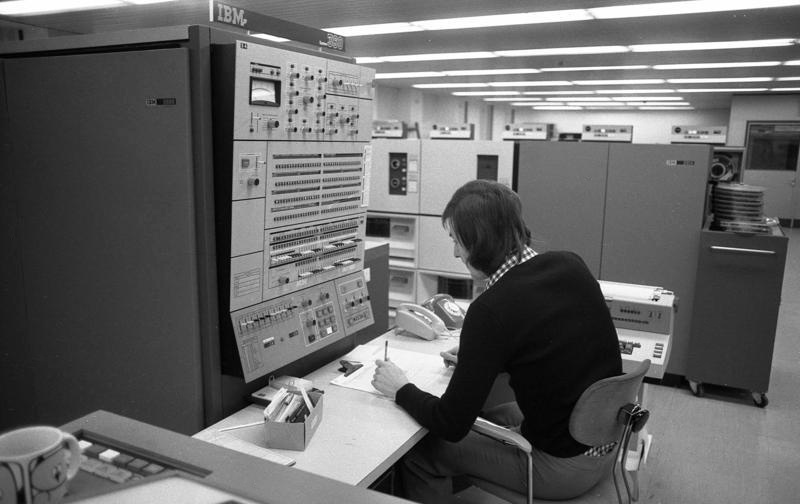
\includegraphics[scale=0.25]
{Photo/Bundesarchiv_B_145_Bild-F038812-0014,_Wolfsburg,_VW_Autowerk.jpg}\\
{\small
ウィキメディア /
Bundesarchiv, B 145 Bild-F038812-0014 / Schaack, Lothar / CC-BY-SA 3.0 de}
\end{myfig}

OS/360を含む第3世代のオペレーティングシステムが
実現した重要な新しい機能を紹介する.

\begin{itemize}
\item {\bf 仮想記憶} \\
主記憶を仮想化し実際より大きい主記憶があるように見せる.
実際の主記憶より大きいプログラムが実行可能になる.

\item {\bf マルチプログラミング} \\
\label{multiprogramming}
\figref{multiprogramming}のように,
複数のプログラム(ジョブ)を主記憶にロードしておき,
その中で実行可能なものを選んで実行する.
入出力待ち等で実行できなくなったら他のプログラムを実行する.
高価なCPUが入出力待ちで停止する可能性を低くすることができた.

\myfigure{btp}{scale=0.66}{Fig/multiprogramming-crop.pdf}
{マルチプログラミングシステム}{multiprogramming}

\item {\bf タイムシェアリング(TSS:Time Sharing System)} \\
マルチプログラミングの一種である.
\figref{timesharing}のように,
複数のターミナルをコンピュータに接続し
複数のユーザが同時にコンピュータを使用できるようにする.
短時間(例えば10ms)で処理するジョブを次々に切り換えることで,
ユーザは自分がコンピュータを独占しているように感じることができる.
なお,ターミナルは\figref{terminal}のような,
キーボードと表示装置だけを備えた安価な装置である.

\myfigure{btp}{scale=0.66}{Fig/timesharing-crop.pdf}
{タイムシェアリングシステム}{timesharing}

\begin{myfig}{btp}{ターミナル}{terminal}
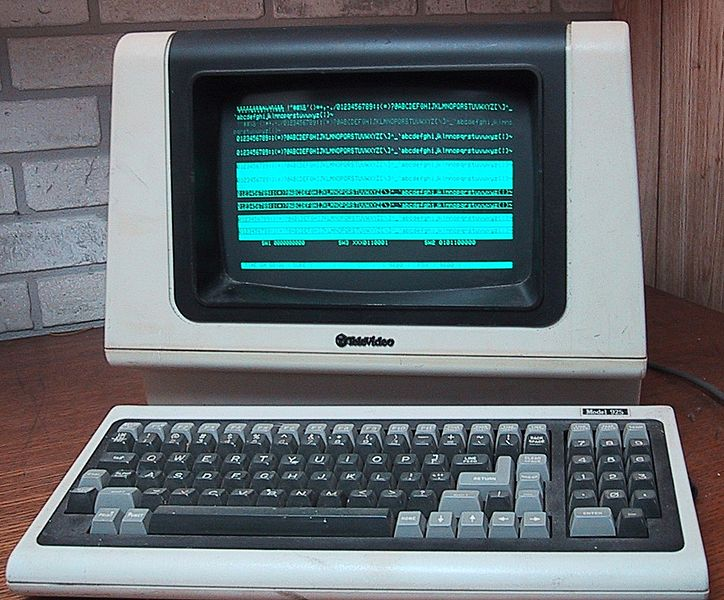
\includegraphics[scale=0.25]{Photo/724px-Televideo925Terminal.jpeg}\\
{\small 写真:
\url{http://commons.wikimedia.org/wiki/File:Televideo925Terminal.jpg}
(パブリックドメイン)}
\end{myfig}

\end{itemize}

この時代のオペレーティングシステムやコンピュータシステム,
そして,それらの開発プロジェクトの中で,
その後のオペレーティングシステムに多くの影響を与えた有名なものを紹介する.

\begin{itemize}
\item OS/360 \\
世界初の本格的な商用オペレーティングシステムである.
メインフレームの主流OSとなり子孫は現在でも使用されている\cite{os360}.

\item MULTICS(MULTiplexed Information and Computing Service)プロジェクト
\cite{third} \\
MIT,ベル研究所,General Electricが共同で始めた
巨大で強力なコンピュータシステムを構築するプロジェクトである.
強力な一台のコンピュータで
都市一つ分のコンピュータサービスを提供する構想だった.
完成までに長い期間を要し(その間にベルとGEが脱落し),
商業的には失敗であったがその後のオペレーティングシステムに影響を与える
多くのアイデアが出てきた.

\item UNIX(ユニックス) \\
MULTICSプロジェクトから抜けたベル研のKen Thompsonらにより開発された
\cite{unix}.
\figref{tree}に示すように,
現代のオペレーティングシステムの多くがUNIXを起源にしている.
子孫ではないものもUNIXの影響を強く受けている.
LinuxはUNIX互換のオペレーティングシステムを作ろうとして
開発が始まった\cite{linux}.
Androidの中身はLinuxである\cite{android}.
z/OSはUNIX互換環境を備えている\cite{zos}.
WindowsにもUNIX互換環境(POSIXサブシステム)を
利用可能なものがある\cite{windows}.

\item DynaBook(ダイナブック:OSだけでなくコンピュータ全体を指す)
\cite{dynabook2} \\
アラン・ケイが1972年に著した
「A Personal Computer for Children of All Ages」\cite{key72, key72J}
に登場する理想のパーソナルコンピュータである.
アラン・ケイがゼロックスのパロアルト研究所に在籍中の1970年代に開発した
Alto上の「暫定ダイナブック環境」(\figref{smalltalk})は
既にGUIやマウスを使用していた.
スティーブ・ジョブスがAltoを見たことが
LISA開発きっかけになったと言われている\cite{dynabook}.

\begin{myfig}{btp}
{Alto(Alto エミュレータ)のスクリーンショット}
{smalltalk}
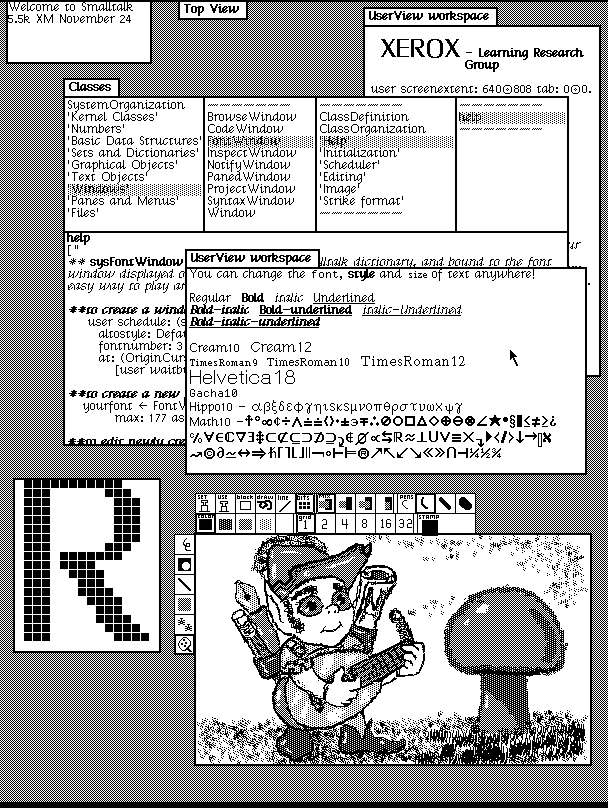
\includegraphics[scale=0.5]{Photo/Smalltalk-76.png}\\
{\small
ウィキメディア /
SUMIM.ST /\\
AltoやNoteTakerで動作した
アラン・ケイ達の暫定Dynabook環境(Smalltalk-76、同-78の頃) /
CC-BY-SA 4.0
}
\end{myfig}

\end{itemize}

\subsection{第4世代(1980〜現代,PCの時代)}

1970年代に単一のLSIにCPU全体を集積したマイクロプロセッサが登場した.
1970年代中旬にはマイクロプロセッサを用いて個人向けのコンピュータである
パーソナルコンピュータ(当時はマイクロコンピュータと呼んでいた)
を作ることが可能になった.
それに伴いパーソナルコンピュータ用のオペレーティングシステムが登場した.

\begin{enumerate}
\item 8bitマイクロコンピュータの時代 \\
1977年にDigtal Reserch社がCP/M(Control Program for Microcomputer)と呼ばれる
8bitマイクロコンピュータ用の簡単なオペレーティングシステムを
開発し成功した.
しかしこのオペレーティングは16bitパーソナルコンピュータの時代には
早々に消え去ってしまった\cite{fourth}.

\item 16bitパーソナルコンピュータの時代 \\
IBMが1981年に16bitパーソナルコンピュータIBM PC\cite{ibmpc81}
(\figref{ibmpc})を発売した.
IBM PCは現在のWindows PCの先祖である.
IBM PCの子孫は改良や拡張を続けながら現在まで高いシェアを維持し続けている.
IBM PCのオペレーティングシステムとして開発されたのが,
Microsoft社のMS-DOS(MicroSoft Disk Operating System)\cite{msdos}である.
バージョン2からはUNIXのような
階層ディレクトリやパイプ,リダイレクト等の機能を持っている.
\figref{tree}に示すように,MS-DOSはWindowsに置き換わりWindows MEまで
バージョンアップが繰り返された.

\begin{myfig}{btp}{IBM PC}{ibmpc}
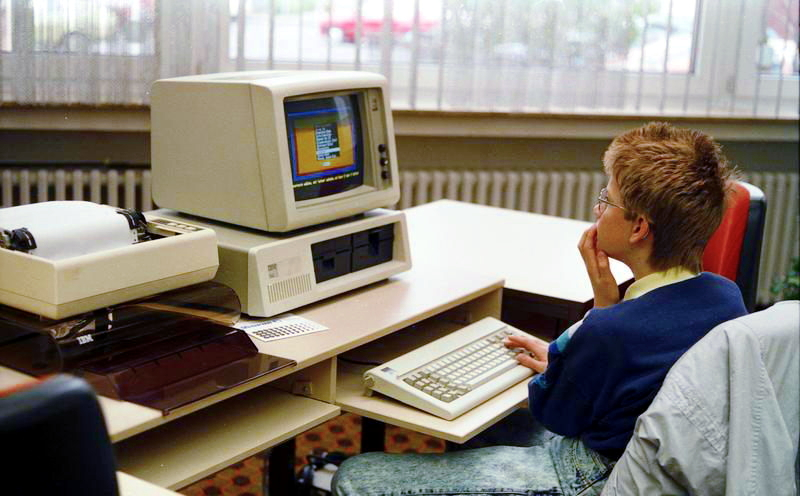
\includegraphics[scale=0.35]
{Photo/Bundesarchiv_B_145_Bild-F077948-0006,_Jugend-Computerschule_mit_IBM-PC.jpg}\\
{\small
ウィキメディア /
Bundesarchiv, B 145 Bild-F077948-0006 / Engelbert Reineke / CC-BY-SA 3.0 de}
\end{myfig}

Apple社は1984年にMacintosh(\figref{macintosh})を発売した.
MachintoshのOSであるMacOSはLISAを経てDynaBook\cite{key72, key72J}の
影響を受けていると言われている\cite{fourth}.
\figref{tree}に示すように,
当初のMacOSはMacOS 9\cite{classicmacos}まで改良が続けられた.

\begin{myfig}{btp}{初代Macintosh}{macintosh}
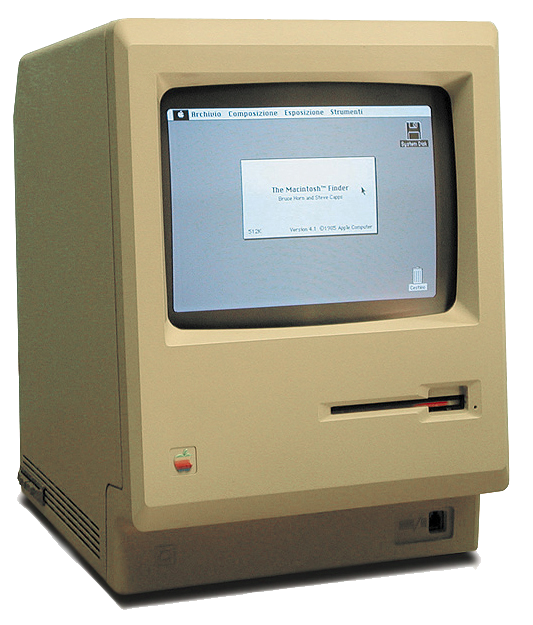
\includegraphics[scale=0.25]{Photo/Macintosh_128k_transparency.png}\\
{\small
ウィキメディア / w:User:Grm wnr / File:Macintosh 128k transparency.png /GFDL}
\end{myfig}

\item 32bitパーソナルコンピュータの時代 \\
1990年頃には32bitのマイクロプロセッサが
パーソナルコンピュータにも使用されるようになった.
32bitのマイクロプロセッサは実行モードを備え,
またメモリ管理ユニットも利用可能であった.
つまり,カーネルモードとユーザモードを使い分けたり
仮想記憶を利用する本格的な第3世代のオペレーティングシステムを
実行できる環境がパーソナルコンピュータにも整った.

そこで,
従来ワークステーションやミニコンで使用されていた
UNIXを安価なパーソナルコンピュータ(特にIBM PC互換機)で
動くようにする人たちが現れ,
オープンソースソフトウェアとしてLinuxやFreeBSD等の開発が始まった.
また,もともとパーソナルコンピュータ用のWindowsやMac OSも
32bitマイクロプロセッサの機能を使いこなす
本格的なオペレーティングシステムに生まれ変わった.

\begin{itemize}
\item Linux \\
1991年に開発が始まったLinuxはUNIX互換のオペレーティングシステムを
パーソナルコンピュータ(IBM PC互換機)用に
独自に作成したものである\cite{linux}.
Linuxは改良され続け,
現在ではパーソナルコンピュータだけでなく,
スーパーコンピュータ「京」のオペレーティングシステム\cite{kei}から,
スマートフォンのオペレーティングシステムであるAndroid\cite{android},
テレビ等の組込みシステムのオペレーティングシステムまで,
広く使われるようになっている.

\item BSD 系の UNIX \\
386BSD\cite{386bsd}はBSD UNIXをIntel 80386 CPUを搭載した
パーソナルコンピュータ(IBM PC互換機)で動作するようにしたものである.
386BSDはFreeBSD等に受継がれるがUNIXのライセンス問題が発生する\cite{unix}.
ライセンス問題が片付き安心して使用できるようになった
4.4BSD-Lite Release 2\cite{unix}をベースに
FreeBSD, NetBSD, OpenBSD 等の多くの BSD 系 PC-UNIXが開発された.

その後,FreeBSDは MacOS X に取り込まれている.
また,FreeBSDにZFSが移植された\cite{zfs}ので
ファイルサーバ用に特化したFreeNAS\cite{freenas}にも使用されている.
なお,徳山工業高等専門学校・情報電子工学科のパソコン室では
1993年10月に386BSDの利用を開始して以来,
2014年3月までFreeBSDを学生用PCやサーバのオペレーティングシステムとして
使用してきた\cite{iebsd}.

\item System V 系の UNIX \\
System V の流れを汲むSolaris\cite{solaris}は,
RISC マイクロプロセッサ SPARC を搭載するサーバやワークステーションでも,
パーソナルコンピュータ(IBM PC 互換)でも使用できる.

\item 従来のパーソナルコンピュータ用オペレーティングシステム \\
従来のWindowsやMac OSはCPUの実行モード等を使用していなかったので,
アプリケーションプログラムのバグにより
システム全体が停止するようなトラブルを防ぐことができなかった.
そこで,32bitマイクロプロセッサの使用を前提に新しく作り直された.

新しく作り直された32bitのWindows NT系列の製品は,
徐々に従来のWindowsを置換えた.
(\figref{tree}参照).
現在(2017年10月)の最新版はWindows 10である.

MacOS は,2001年にUNIXの流れを汲み安定して動作するOPENSTEPベースの
MacOS X\cite{macos}に置き換わった(\figref{tree}参照).
その後,名称が OS X, macOS と変更されたがこれらは MacOS X の改良版である.
現在(2017年10月)の最新版はmacOS 10.13 High Sierraである.
iPhoneのiOSはMacOS Xをタッチパネル用に再構成したものである\cite{ios}.
\end{itemize}
\end{enumerate}

\subsection{インターネット世代}
現在のオペレーティングシステムはTCP/IP機構が組込まれ
インターネットに接続することができる.
今ではパーソナルコンピュータやスマートフォンの使用を
インターネット抜きに考えることができない.
オペレーティングシステムにとってインターネットに接続できることは
重要なことである.

TCP/IPを実装した4.2BSDが1984年に公開された\cite{bsd}.
以来,4.2BSDの子孫はインターネットに対応している.
1988年に公開されたSystem V R4はBSD起原のTCP/IPの実装を含んでいた\cite{svr4}.
これの子孫もインターネットに対応している.
Linuxも1.0の頃にはTCP/IPの実装を含んでいた\cite{linux1}.
WindowsはWindows 95からTCP/IPを標準装備している\cite{windows}.
MacOSはMacOS 8が発表されるまでにはインターネット対応がされていた
\cite{classicmacos}.
メインフレームの世界でもOS/390はインターネットに対応した\cite{os390}.

このようにして1990年代の後半には多くのオペレーティングシステムが
インターネット対応を完了させた.
インターネット対応を完了させたオペレーティングシステムを
「インターネット世代のオペレーティングシステム」と言うことができる.

\begin{myfig}{btp}{オペレーティングシステムの系統図}{tree}
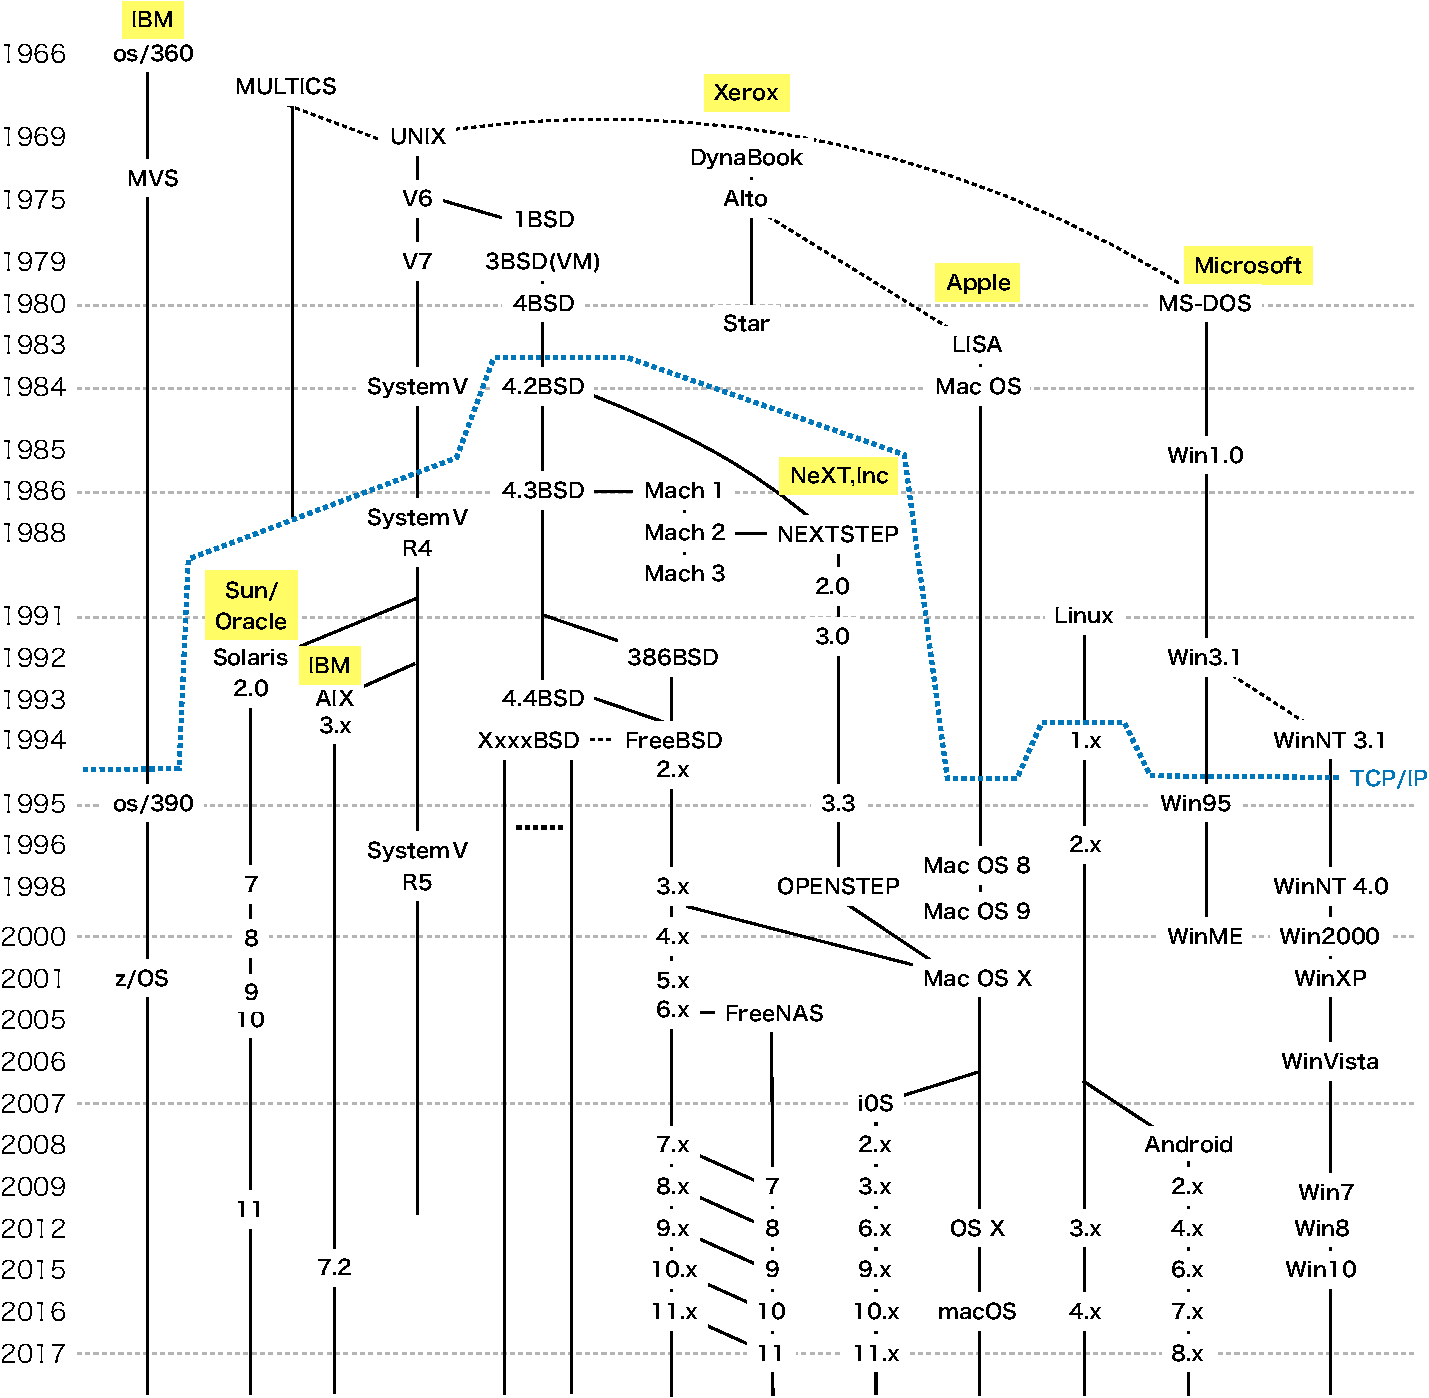
\includegraphics[scale=0.6]{Fig/tree-crop.pdf}\\
{\small
系統図は\cite{os360,
mvs,
os390,
zos,
unix,
solaris,
aix,
mach,
bsd,
bsdd,
386bsd,
freebsd,
freenas,
nextstep,
classicmacos,
dynabook,
macos,
ios,
linux,
android,
msdos,
windows}
の内容を総合して作成した.}
\end{myfig}
